\documentclass[twoside]{book}

% Packages required by doxygen
\usepackage{fixltx2e}
\usepackage{calc}
\usepackage{doxygen}
\usepackage[export]{adjustbox} % also loads graphicx
\usepackage{graphicx}
\usepackage[utf8]{inputenc}
\usepackage{makeidx}
\usepackage{multicol}
\usepackage{multirow}
\PassOptionsToPackage{warn}{textcomp}
\usepackage{textcomp}
\usepackage[nointegrals]{wasysym}
\usepackage[table]{xcolor}

% Font selection
\usepackage[T1]{fontenc}
\usepackage[scaled=.90]{helvet}
\usepackage{courier}
\usepackage{amssymb}
\usepackage{sectsty}
\renewcommand{\familydefault}{\sfdefault}
\allsectionsfont{%
  \fontseries{bc}\selectfont%
  \color{darkgray}%
}
\renewcommand{\DoxyLabelFont}{%
  \fontseries{bc}\selectfont%
  \color{darkgray}%
}
\newcommand{\+}{\discretionary{\mbox{\scriptsize$\hookleftarrow$}}{}{}}

% Page & text layout
\usepackage{geometry}
\geometry{%
  a4paper,%
  top=2.5cm,%
  bottom=2.5cm,%
  left=2.5cm,%
  right=2.5cm%
}
\tolerance=750
\hfuzz=15pt
\hbadness=750
\setlength{\emergencystretch}{15pt}
\setlength{\parindent}{0cm}
\setlength{\parskip}{3ex plus 2ex minus 2ex}
\makeatletter
\renewcommand{\paragraph}{%
  \@startsection{paragraph}{4}{0ex}{-1.0ex}{1.0ex}{%
    \normalfont\normalsize\bfseries\SS@parafont%
  }%
}
\renewcommand{\subparagraph}{%
  \@startsection{subparagraph}{5}{0ex}{-1.0ex}{1.0ex}{%
    \normalfont\normalsize\bfseries\SS@subparafont%
  }%
}
\makeatother

% Headers & footers
\usepackage{fancyhdr}
\pagestyle{fancyplain}
\fancyhead[LE]{\fancyplain{}{\bfseries\thepage}}
\fancyhead[CE]{\fancyplain{}{}}
\fancyhead[RE]{\fancyplain{}{\bfseries\leftmark}}
\fancyhead[LO]{\fancyplain{}{\bfseries\rightmark}}
\fancyhead[CO]{\fancyplain{}{}}
\fancyhead[RO]{\fancyplain{}{\bfseries\thepage}}
\fancyfoot[LE]{\fancyplain{}{}}
\fancyfoot[CE]{\fancyplain{}{}}
\fancyfoot[RE]{\fancyplain{}{\bfseries\scriptsize Generated by Doxygen }}
\fancyfoot[LO]{\fancyplain{}{\bfseries\scriptsize Generated by Doxygen }}
\fancyfoot[CO]{\fancyplain{}{}}
\fancyfoot[RO]{\fancyplain{}{}}
\renewcommand{\footrulewidth}{0.4pt}
\renewcommand{\chaptermark}[1]{%
  \markboth{#1}{}%
}
\renewcommand{\sectionmark}[1]{%
  \markright{\thesection\ #1}%
}

% Indices & bibliography
\usepackage{natbib}
\usepackage[titles]{tocloft}
\setcounter{tocdepth}{3}
\setcounter{secnumdepth}{5}
\makeindex

% Hyperlinks (required, but should be loaded last)
\usepackage{ifpdf}
\ifpdf
  \usepackage[pdftex,pagebackref=true]{hyperref}
\else
  \usepackage[ps2pdf,pagebackref=true]{hyperref}
\fi
\hypersetup{%
  colorlinks=true,%
  linkcolor=blue,%
  citecolor=blue,%
  unicode%
}

% Custom commands
\newcommand{\clearemptydoublepage}{%
  \newpage{\pagestyle{empty}\cleardoublepage}%
}

\usepackage{caption}
\captionsetup{labelsep=space,justification=centering,font={bf},singlelinecheck=off,skip=4pt,position=top}

%===== C O N T E N T S =====

\begin{document}

% Titlepage & ToC
\hypersetup{pageanchor=false,
             bookmarksnumbered=true,
             pdfencoding=unicode
            }
\pagenumbering{alph}
\begin{titlepage}
\vspace*{7cm}
\begin{center}%
{\Large Libres\+Doxy }\\
\vspace*{1cm}
{\large Generated by Doxygen 1.8.14}\\
\end{center}
\end{titlepage}
\clearemptydoublepage
\pagenumbering{roman}
\tableofcontents
\clearemptydoublepage
\pagenumbering{arabic}
\hypersetup{pageanchor=true}

%--- Begin generated contents ---
\chapter{Hierarchical Index}
\section{Class Hierarchy}
This inheritance list is sorted roughly, but not completely, alphabetically\+:\begin{DoxyCompactList}
\item \contentsline{section}{Administrador}{\pageref{class_administrador}}{}
\item P\+DO\begin{DoxyCompactList}
\item \contentsline{section}{Conexion}{\pageref{class_conexion}}{}
\end{DoxyCompactList}
\end{DoxyCompactList}

\chapter{Data Structure Index}
\section{Data Structures}
Here are the data structures with brief descriptions\+:\begin{DoxyCompactList}
\item\contentsline{section}{\mbox{\hyperlink{class_administrador}{Administrador}} }{\pageref{class_administrador}}{}
\item\contentsline{section}{\mbox{\hyperlink{class_conexion}{Conexion}} }{\pageref{class_conexion}}{}
\end{DoxyCompactList}

\chapter{Data Structure Documentation}
\hypertarget{class_administrador}{}\section{Administrador Class Reference}
\label{class_administrador}\index{Administrador@{Administrador}}
\subsection*{Public Member Functions}
\begin{DoxyCompactItemize}
\item 
\mbox{\Hypertarget{class_administrador_a12251d0c022e9e21c137a105ff683f13}\label{class_administrador_a12251d0c022e9e21c137a105ff683f13}} 
{\bfseries get\+Id} ()
\item 
\mbox{\Hypertarget{class_administrador_a38abe751ca21ffb95d9c90862e0fb96f}\label{class_administrador_a38abe751ca21ffb95d9c90862e0fb96f}} 
{\bfseries get\+Usuario} ()
\item 
\mbox{\Hypertarget{class_administrador_a435e52a33b28962d26d59ff9fc36139a}\label{class_administrador_a435e52a33b28962d26d59ff9fc36139a}} 
{\bfseries get\+Contrasenia} ()
\item 
\mbox{\Hypertarget{class_administrador_a589f85a7401ec0dde7cb329d87b14677}\label{class_administrador_a589f85a7401ec0dde7cb329d87b14677}} 
{\bfseries get\+Tipo} ()
\item 
\mbox{\Hypertarget{class_administrador_aee7a5f0ec54dd116afc50da524b2a43e}\label{class_administrador_aee7a5f0ec54dd116afc50da524b2a43e}} 
{\bfseries get\+Esta\+Activo} ()
\item 
\mbox{\Hypertarget{class_administrador_a87313ad678fb2a2a8efb435cf0bdb9a0}\label{class_administrador_a87313ad678fb2a2a8efb435cf0bdb9a0}} 
{\bfseries set\+Id} (\$id)
\item 
\mbox{\Hypertarget{class_administrador_a48255b4550c8d4dc7aedf7837439461a}\label{class_administrador_a48255b4550c8d4dc7aedf7837439461a}} 
{\bfseries set\+Usuario} (\$usuario)
\item 
\mbox{\Hypertarget{class_administrador_ae1ceda2bd81bed0d084e2a5862e43e1e}\label{class_administrador_ae1ceda2bd81bed0d084e2a5862e43e1e}} 
{\bfseries set\+Contrasenia} (\$contrasenia)
\item 
\mbox{\Hypertarget{class_administrador_affc705d55128668ebea5660dcde63ada}\label{class_administrador_affc705d55128668ebea5660dcde63ada}} 
{\bfseries set\+Tipo} (\$tipo)
\item 
\mbox{\Hypertarget{class_administrador_ac6dda1558ef944e2adfc76a014dc0f0c}\label{class_administrador_ac6dda1558ef944e2adfc76a014dc0f0c}} 
{\bfseries set\+Esta\+Activo} (\$esta\+Activo)
\item 
\mbox{\Hypertarget{class_administrador_ab0c2edaf3b8fc9898f74d2cd821acaaa}\label{class_administrador_ab0c2edaf3b8fc9898f74d2cd821acaaa}} 
{\bfseries \+\_\+\+\_\+construct} (\$usuario, \$contrasenia, \$tipo=\textquotesingle{}A\+DM\textquotesingle{}, \$esta\+Activo=\textquotesingle{}V\textquotesingle{}, \$id=null)
\item 
\mbox{\Hypertarget{class_administrador_a7eff1139ff047569a4d8bff22dfaee0c}\label{class_administrador_a7eff1139ff047569a4d8bff22dfaee0c}} 
{\bfseries guardar} ()
\item 
\mbox{\Hypertarget{class_administrador_a804dc6dc2fe1206778036ac9bf6f4947}\label{class_administrador_a804dc6dc2fe1206778036ac9bf6f4947}} 
{\bfseries presentar\+Admins} ()
\end{DoxyCompactItemize}
\subsection*{Static Public Member Functions}
\begin{DoxyCompactItemize}
\item 
\mbox{\Hypertarget{class_administrador_a44bf2207d08435f206481d8e4358876a}\label{class_administrador_a44bf2207d08435f206481d8e4358876a}} 
static {\bfseries buscar\+Por\+Id} (\$id)
\end{DoxyCompactItemize}
\subsection*{Data Fields}
\begin{DoxyCompactItemize}
\item 
\mbox{\Hypertarget{class_administrador_ac0414ee341593c7a07644267c5c67728}\label{class_administrador_ac0414ee341593c7a07644267c5c67728}} 
const {\bfseries tabla} = \textquotesingle{}usuario\textquotesingle{}
\end{DoxyCompactItemize}


The documentation for this class was generated from the following file\+:\begin{DoxyCompactItemize}
\item 
C\+:/xampp/htdocs/git/sistemadegestiondeobjetosdeaprendizaje/sgoa/aplicacion/clases\+\_\+negocio/clase\+\_\+administrador.\+php\end{DoxyCompactItemize}

\hypertarget{class_conexion}{}\section{Conexion Class Reference}
\label{class_conexion}\index{Conexion@{Conexion}}
Inheritance diagram for Conexion\+:\begin{figure}[H]
\begin{center}
\leavevmode
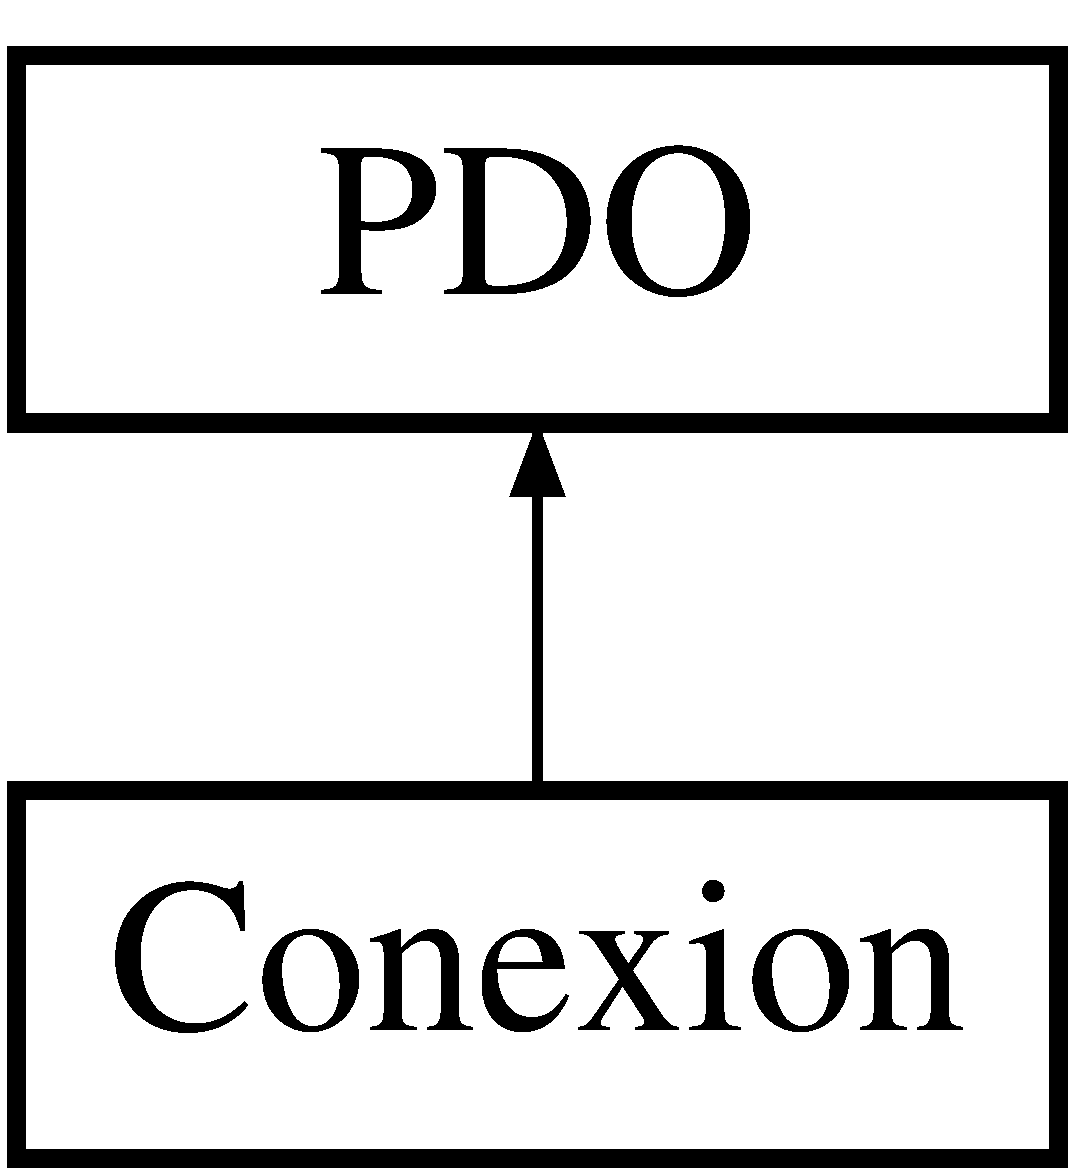
\includegraphics[height=2.000000cm]{class_conexion}
\end{center}
\end{figure}


The documentation for this class was generated from the following file\+:\begin{DoxyCompactItemize}
\item 
C\+:/xampp/htdocs/git/sistemadegestiondeobjetosdeaprendizaje/sgoa/aplicacion/clases\+\_\+negocio/clase\+\_\+conexion.\+php\end{DoxyCompactItemize}

%--- End generated contents ---

% Index
\backmatter
\newpage
\phantomsection
\clearemptydoublepage
\addcontentsline{toc}{chapter}{Index}
\printindex

\end{document}
